% Acertar titulo do capitulo

A internet apresenta um crescimento exponencial no mundo atual.
Estima-se que no ano de 2016 cerca de 66\% da população brasileira tenha acesso à rede \cite{social17}.
Ela é usada massivamente no dia a dia das pessoas, estando presente desde a realização de tarefas básicas e essenciais,
como cozinhar e se locomover numa cidade, até o preenchimento do tempo de lazer, com vídeos, notícias, mensagens
instantâneas e redes sociais.
% Falar sobre o uso da internet, ubuiquidade e etc

Através especialmente das redes sociais, a internet modificou a forma de interação entre as pessoas.
No Brasil, 58\% da população, ou seja, 120 milhões de pessoas, participam de pelo menos uma rede social, gastando em
média 220 minutos por dia~\cite{social17}.
Isso faz do Brasil o segundo país em tempo navegando em redes sociais, atrás apenas das Filipinas~\cite{social17}.
Isso não só cria uma nova instância de comunicação entre as pessoas, mas também abre um lugar para a expressão dos
sentimentos e opiniões de cada um.
Com isso, após o surgimento das redes sociais, a presença online deixou de ser uma comunicação de via única.
Agora, os leitores interagem com a fonte de informação recebida, seja ela uma notícia, atualização de amigos, etc.

Essa presença central das mídias sociais na vida das pessoas faz com que os usuários passem a ser mais influenciados
por opiniões que trafegam pela mesma.
Desta maneira, as redes sociais passam a ter um peso maior na tomada de decisão de cada individuo, como na compra de
um produto ou na escolha de um candidato para a ser votado.
O impacto destes novos meios de comunicação podem ser observados, por exemplo, nas mobilizações de massa ocorridas na
primavera árabe em 2011 que levaram a queda de governos no qual as mídias sociais exerceram papel
crítico~\cite{mourtada11}.

Nesse sentido, tornaram-se necessários trabalhos que analisem o que se está dizendo nas redes sociais.
Para uma emissora de TV, por exemplo, é interessante saber o que está sendo dito sobre sua programação, assim como para
a assessoria de um cantor, é importante descobrir se sua nova canção está agradando ou não seu público.

Entretanto, a criação de conteúdo digital acompanha o crescimento da internet.
No ano de 2016, a cada sessenta segundos foram adicionadas 500 horas vídeo no YouTube, realizadas 3.8 milhões de buscas
no Google e publicados 450 mil \textit{tweets}~\cite{smartinsights}.
Pode-se observar que se torna impraticável a realização de análise de sentimento manualmente sobre mídias com esse volume
de dados.
Portanto, a utilização de métodos de aprendizado de máquina é um modo de viabilizar a realização dessa tarefa.

Jim Yu, presidente da empresa de marketing digital BrightEdge, ressalta que os sentimentos expressados por clientes em
relação a uma marca é uma das principais métricas de \textit{branding}~\cite{marketingland}.
O colunista da Forbes, Daniel Newman, destaca que a utilização desta e outras técnicas de big data vem revolucionando
a forma de se fazer marketing, permitindo uma maior personalização dos produtos e fortalecimento de relação com os
clientes.
Além de ser utilizada como métrica de relações comerciais, análises de sentimento de mídias sociais são aplicadas na
predição de mercados financeiros~\cite{bollen11}, na predição de resultados eleitorais~\cite{tumasjan10}, entre outros.

\section{Análise de Sentimento}

O campo de estudos da análise de sentimento, também chamado de mineração de opinião, é um dos ramos mais ativos do
processamento de linguagem natural~\cite{liu12}.
A análise de sentimento visa analisar a opinião, a avaliação, a emoção e  a atitude de um documento em relação a um
evento, produto, serviço, organização, etc.
Apesar do processamento de linguagem natural ter um longo histórico de estudos, a análise de sentimento se consolidou
apenas no inicio dos anos 2000 com a crescente demanda comercial.
Observa-se que o crescimento de interesse nessa área tem grande correlação com o crescimento de mídias sociais e do
volume de dados, visto que o sucesso das redes sociais disponibilizam quantidades massivas de dados possibilitando o
desenvolvimento de técnicas quanto oferecem oportunidades de aplicações~\cite{liu12}.

O campo de análise de sentimento apresenta diferentes subáreas de estudo.
Dentre elas, a tarefa mais presente na literatura e que abordaremos neste trabalho é a análise de polaridade de um
documento.
A análise de polaridade visa classificar textos em uma escala entre positivo e negativo.
Encontra-se também estudos que visam determinar a subjetividade ou objetividade de um texto, como no trabalho de Wiebe e
Rilof~\cite{Wiebe05}.
Também entra no escopo de análise de sentimento a classificação de emoções presentes em uma mensagem, como felicidade,
raiva, tristeza, etc.
Outro foco de pesquisa com grande aplicações práticas é a análise de sentimento porém não da mensagem como um todo, mas
do sentimento em relação a uma entidade presente na mensagem.
O contrário também é possível, a análise da influência de sentimento de um termo em relação a mensagem.
Percebe-se que a análise de sentimento se desmembra em varias subdivisões, novas subdivisões surgem a cada dia visto que
a área ainda está em sua infância, o que confirma seu grande potencial de aplicação.

A tabela~\ref{tab:sentiment} exemplifica a classificação de polaridade de \textit{tweets}, foco deste trabalho.

\begin{table}[h]
    \begin{center}
        \begin{tabular}{| l | p{10cm} |}
        \hline
        \textbf{Sentimento} & \textbf{\textit{Tweet}} \\ \hline
        Positivo & Grande notícia, João Sousa e Gastão Elias representam Portugal nos Jogos Olímpicos do Rio de Janeiro.
        \\ \hline
        Neutro & Entrevistei hoje a Priscilla Carnaval do BMX. Classificada para o \#Rio2016, ela tem novidades na
        preparação olímpica. \\ \hline
        Negativo & Estão transformando Olimpíadas que é algo sério num espetáculo triste e de mau gosto. \\ \hline
        \end{tabular}
        \caption{Exemplo de classificação de sentimento em \textit{tweets}.}
    \end{center}
    \label{tab:sentiment}
\end{table}

% falar de tecnicas com papers utilizados
% (revisão bibliografica)

\section{Twitter}

O Twitter é um microblog e rede social no qual os usuários interagem a partir de mensagens, chamadas \textit{tweets}.
Microblogs são meios de comunicação que permitem usuários a compartilhar conteúdos e mídias.
As principais características dos microblogs são a brevidade e instantaneidade.
Os \textit{tweets} são limitados a 140 caracteres e podem conter fotos, vídeos, links, localizações referências a
usuários e \textit{hashtags}.
Criado em 2006, o site cresceu rapidamente a ponto de se tornar uma redes sociais com maior número de usuários no mundo.
No ano de 2016 o Twitter a plataforma obteve a presença de 330 milhões de usuários ativos por mês.

Um ponto chave da comunicação por Twitter são as \textit{hashtags}.
\textit{Hashtags} são palavras-chave ou frases que definem um tópico ou tema.
Elas são caracterizadas por serem precedidas pelo simbolo da tralha (\#) e por não conterem espaços ou pontuação, como
ilustrado na figura~\ref{fig:hashtag}.
São, ainda, elementos clicáveis que apontam o leitor para outra página.
Essa outra página, por sua vez, contém um mural com todas as citações contendo aquela \textit{hashtag}.
Desta forma, \textit{hashtags} funcionam como agregadores de \textit{tweets}.

\begin{figure}
\begin{center} {
    \begin{center}
    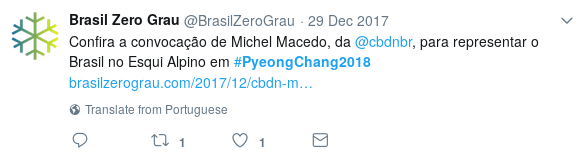
\includegraphics[scale=0.7]{tweet-hashtag.png}
    \caption{Exemplo de \textit{tweet} com a utilização de \textit{hashtag}.}
    \label{fig:hashtag}
    \end{center}
}
\end{center}
\end{figure}

O tamanho reduzido das mensagens veiculadas por Twitter e o meio pelo qual elas circulam levam a utilização de
variações gramaticais da língua especificas para este ambiente.
É comum encontrar, por exemplo, o uso excessivo de abreviações para reduzir a contagem total de caracteres, a repetição
de pontuação para reforçar intensidade e o uso de neologismos.

Se tratando de classificação de sentimento, o fato do tamanho reduzido e linguagem própria apresentam uma dificuldade
adicional.
Outro traço notável é que por ser uma plataforma aberta, o Twitter é composto de mensagens dos mais diversos domínios.
Esse fator dificulta a tarefa a ser executada quando comparado com trabalhos de um domínio específico, como por exemplo
a análise de sentimento para avaliação de filmes a partir de resenhas; ou na predição de flutuações do mercado
financeiro pela análise de artigos jornalísticos.
Apesar de não serem abordadas nesse trabalho, atributos não textuais como: republicação ou citação de mensagem, presença
de foto ou vídeo, grafos de conexões entre usuários etc podem colaborar na realização da tarefa de análise de sentimento.
